\chapter{Determinación de la solución óptima}
\minitoc

Para poder evaluar la mejor de las soluciones, así como determinar la altura orbital óptima para nuestra misión, se va a realizar una simulación que estime la masa total de las posibles soluciones de satélite. 
El procedimiento es el siguiente:

\begin{enumerate}
    \item Se estimará la masa en seco del satélite (es decir, sin contar con su combustible), así como volumen, superficie y potencia eléctrica requerida por el instrumento. 
    \item Se establecerá un modelo de decaimiento orbital que calcule el numero de impulsos, Delta-V y combustible total utilizado para el mantenimiento de la órbita
    \item Se agregarán ambos resultados que, cruzados, darán la masa mínima del satélite necesario, que será la solución óptima.
\end{enumerate}

\newpage
\section{Estimación de la masa seca }

El libro \textit{System Mission Analysis and Design} (1999, 3a Ed) \cite{wertz1999smad}, en su capítulo 9.5 , define una forma de estimar la masa del instrumento, así como del satélite, en función de otros instrumentos con diámetros de pupilas y masas conocidos. Dichas ecuaciones son:

%% ECUACIONES
\begin{equation}
\begin{gathered}
R = \frac{A_i}{A_o}; \quad L_i = R \cdot L_o; \quad S_i = L_i^2; \quad V_i = L_i^3 \\
W_i = K \cdot R^3 \cdot W_o; \quad P_i = K \cdot R^3 \cdot P_o
\end{gathered}
\end{equation}

\begin{itemize}
    \item El subíndice $i$ indica el parámetro de la misión actual, mientras que el subíndice $o$ será el el parámetro de la misión de referencia. 
    \item $A, L, S, V, W, P$ definen, respectivamente el diámetro, longitud, superficie, volumen, masa y potencia eléctrica del instrumento.
    \item Se define el factor $K$ como $1$ cuando $R\geq 0,5$. En caso contrario se establece $K=2$.
\end{itemize}
Usando datos de otras misiones proporcionadas por el tutor (THEMATIC MAPPER Y SEOSAT) se realizará el cálculo interpolando los resultados de las estimaciones entre ambas misiones.

\begin{table}[H]
    \centering
    \caption{Instrumentos de referencia para la estimación por escalado. \\ Fuente: \cite{zorita_dimensiones_2023}.}
    \begin{tabular}{@{}lll@{}}
        \toprule
        Parámetro     & Thematic Mapper       & SEOSAT Primary Payload \\
        \midrule
        Dimensiones   & 2\,m × 1\,m × 1\,m     & 1\,m × 1\,m × 1\,m      \\
        Masa          & 240\,kg                & 100\,kg                \\
        Consumo       & 280\,W                 & 100\,W                 \\
        Pupila        & 0.4\,m                 & 0.25\,m                \\
        \bottomrule
    \end{tabular}
    
\end{table}

Asumiendo además que la masa del instrumento es un 25\% de la masa del satélite, que un telescopio adicional aumenta la masa del instrumento en un 50\% \cite{zorita_dimensiones_2023}, y utilizando como \textit{input} la relación $h\ vs\ D_{min}$ extraída previamente, se obtienen los siguientes resultados:

% TABLA PESO POTENCIA 
\begin{figure}[H]
    \centering
    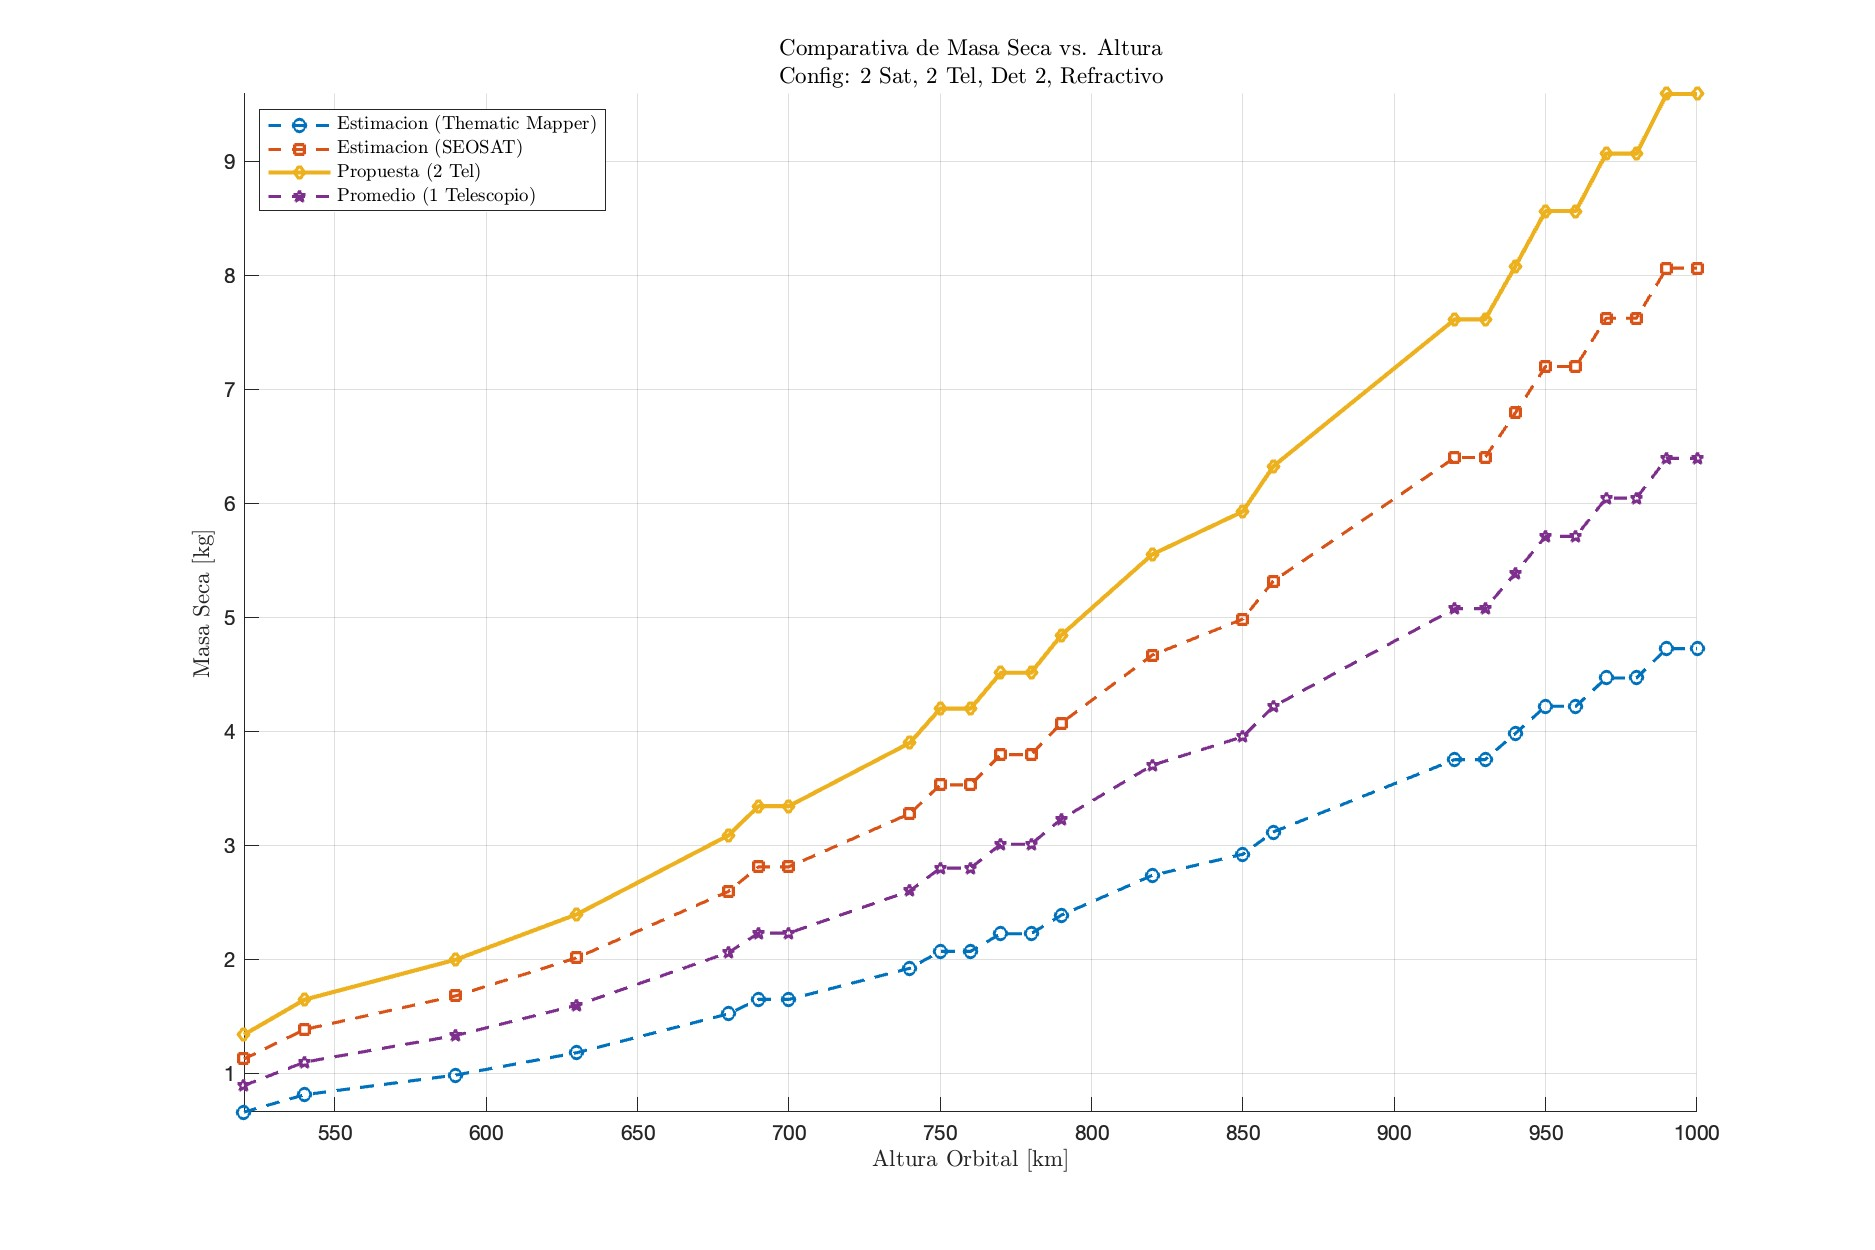
\includegraphics[width=1\linewidth]{5.Mission/MasaSeca_Comparativa_2sat_2tel_Det2_Refractivo.jpg}
    \caption{Estimación de la masa seca del satélite en función de la altura. \\Fuente: Elaboración propia.}
    \label{masaseca}
\end{figure}

Aparecen, en la figura \ref{masaseca}, las estimaciones  de masa seca realizadas con los puntos extraídos de la relación $h\ vs\ D_{min}$, mediante THEMATIC MAPPER y mediante SEOSAT, junto con su promedio. La relación propuesta (en amarillo) aumentará un 50\% sobre este promedio al tener un telescopio adicional.

\section{Impulsos, $\Delta V$ y masa de combustible. Fin de misión. }

Para calcular la masa de combustible necesaria para mantener la misión durante los 8 años requeridos, se debe realizar un modelo de cálculo de arrastre atmosférico.

\subsection{Modelado Arrastre atmosférico}

La variación temporal del semieje mayor \(a= R_T+h\) debida al arrastre se modela mediante
\begin{equation}
\frac{\mathrm d a}{\mathrm d t}=-
\frac{C_{d}\,A\,\rho(h)\,\sqrt{\mu\,a}}{m},
\label{eq:dadt}
\end{equation}
donde \(C_{d}\) es el coeficiente de arrastre, \(A\) el área frontal efectiva calculada anteriormente, 
\(m\) la masa del satélite y \(\mu\) el parámetro gravitacional terrestre. Se tomará un $C_d = 2,5$ \cite{cook1965satellite}.
La densidad \(\rho(h)\) se aproxima con un modelo exponencial por capas, basado en la Atmósfera Estándar de Estados Unidos 1976 (USSA76) \cite{usstandardatmosphere1976}:  
\begin{equation}
\rho(h)=\rho_{0}\,
\exp\!\Bigl[-\dfrac{h-h_{\text{base}}}{H}\Bigr],
\end{equation}
siendo \(\rho_{0}\) la densidad tabulada a la base de cada capa, de 50 km y \(H\) su altura
de escala \cite{vallado2013fundamentals}.  


\subsection{Cálculo del Delta-V, número de impulsos y masa de
combustible}\label{sec:deltav}

Para calcular el decaimiento orbital se resuelve numéricamente la ecuación~\eqref{eq:dadt}  con el \textit{solver} nativo de MATLAB \texttt{ode45}. Imponiendo que, cuando la altura actual caiga por debajo del 98\% de la altura objetivo inicial, realiza un impulso, devolviendo el satélite a dicha altura. Tras ello, calcula el delta-V necesario. Esta maniobra se ejecuta como un re‐empuje mediante una transferencia de Hohmann entre los radios \cite{curtis2020orbital}:
\(\,r_{1}=R_{\oplus}+h_{\text{actual}}\) y
\(r_{2}=R_{\oplus}+h_{\text{objetivo}}\).  
El incremento de velocidad por maniobra es
\begin{equation}
\Delta v =
\left(\sqrt{\frac{\mu}{r_{1}}}\,
      \bigl[\sqrt{2r_{2}/(r_{1}+r_{2})}-1\bigr]\right)
+
\left(\sqrt{\frac{\mu}{r_{2}}}\,
      \bigl[1-\sqrt{2r_{1}/(r_{1}+r_{2})}\bigr]\right).
\label{eq:dv_hohmann}
\end{equation}

\begin{figure}[H]
    \centering
    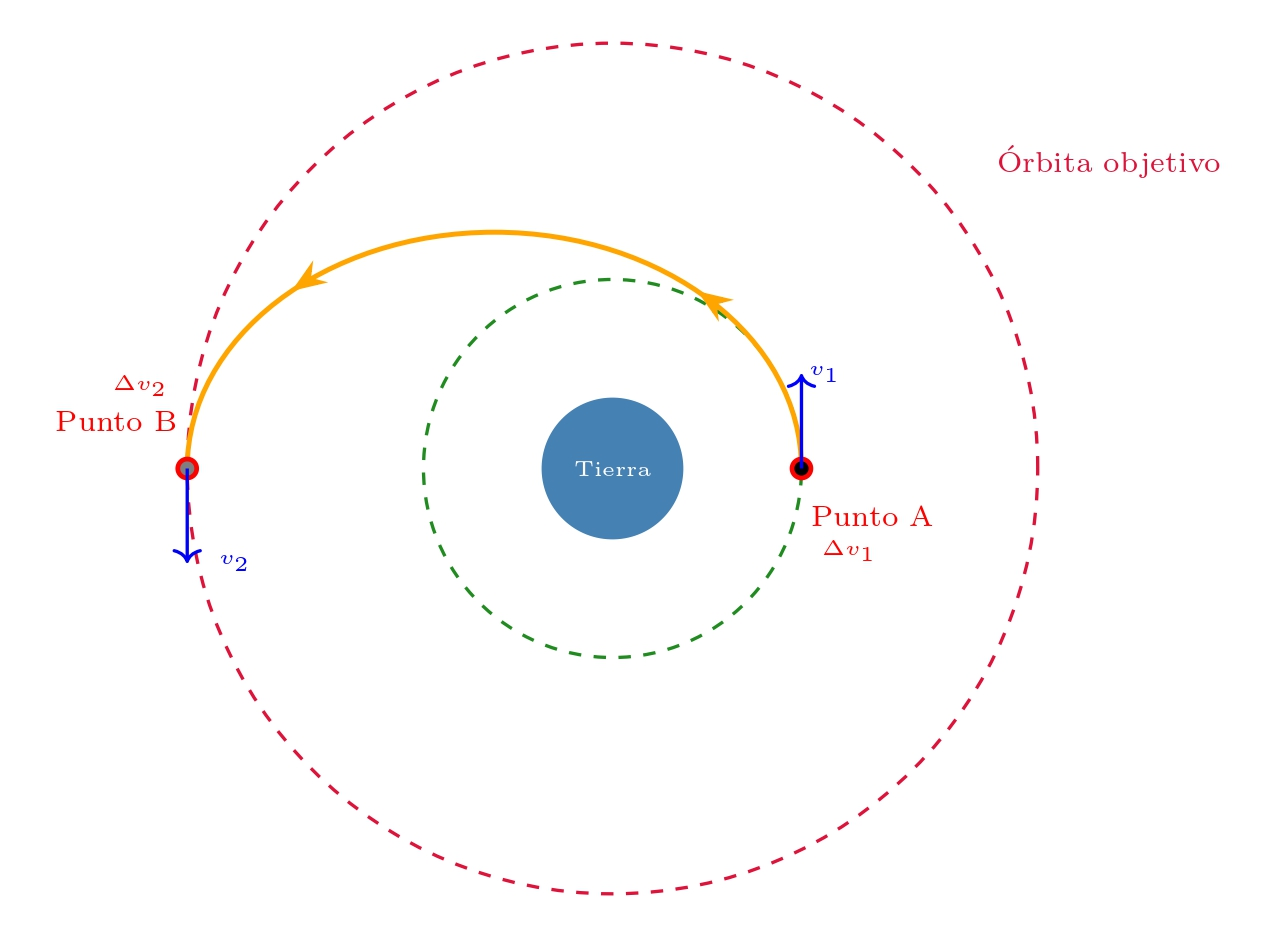
\includegraphics[width=0.5\linewidth]{5.Mission/TFG_Tikz_7.jpg}
    \caption{Transferencia de Hohmann. \\Fuente: Elaboración propia.}
    \label{fig:enter-label}
\end{figure}

El proceso iterativo continúa durante la vida nominal de la misión
(\(T = 8\)~años).  
Se acumulan el número de impulsos \(N\) y el \(\Delta v_{\text{tot}}\)
empleado.  
Concluida la simulación, la masa de combustible se obtiene aplicando la ecuación de Tsiolkovski \cite{curtis2020orbital}:
\begin{equation}
m_{\text{prop}} = m_{\text{seca}}
\left(\exp\!\Bigl[\frac{\Delta v_{\text{tot}}}{I_{sp}\,g_{0}}\Bigr]-1\right),
\label{eq:tsiolkovsky}
\end{equation}
donde se estima el impulso específico inicial\(I_{sp}= 220s\)  y
\(g_{0}=9.80665\ \mathrm{m\,s^{-2}}\).
Además, se añade un margen del 10\% para contingencias:
\(
m_{\text{prop,\,final}}=1.1\,m_{\text{prop}}
\),
de modo que la masa total del satélite resulta
\(m_{\text{total}} = m_{\text{seco}} + m_{\text{prop,\,final}}\).


Una vez calculada la masa de combustible para todos los posibles puntos de altura, se suma a la masa seca estimada previamente, obteniendo la masa total en función de la altura:

\begin{figure}[H]
    \centering
    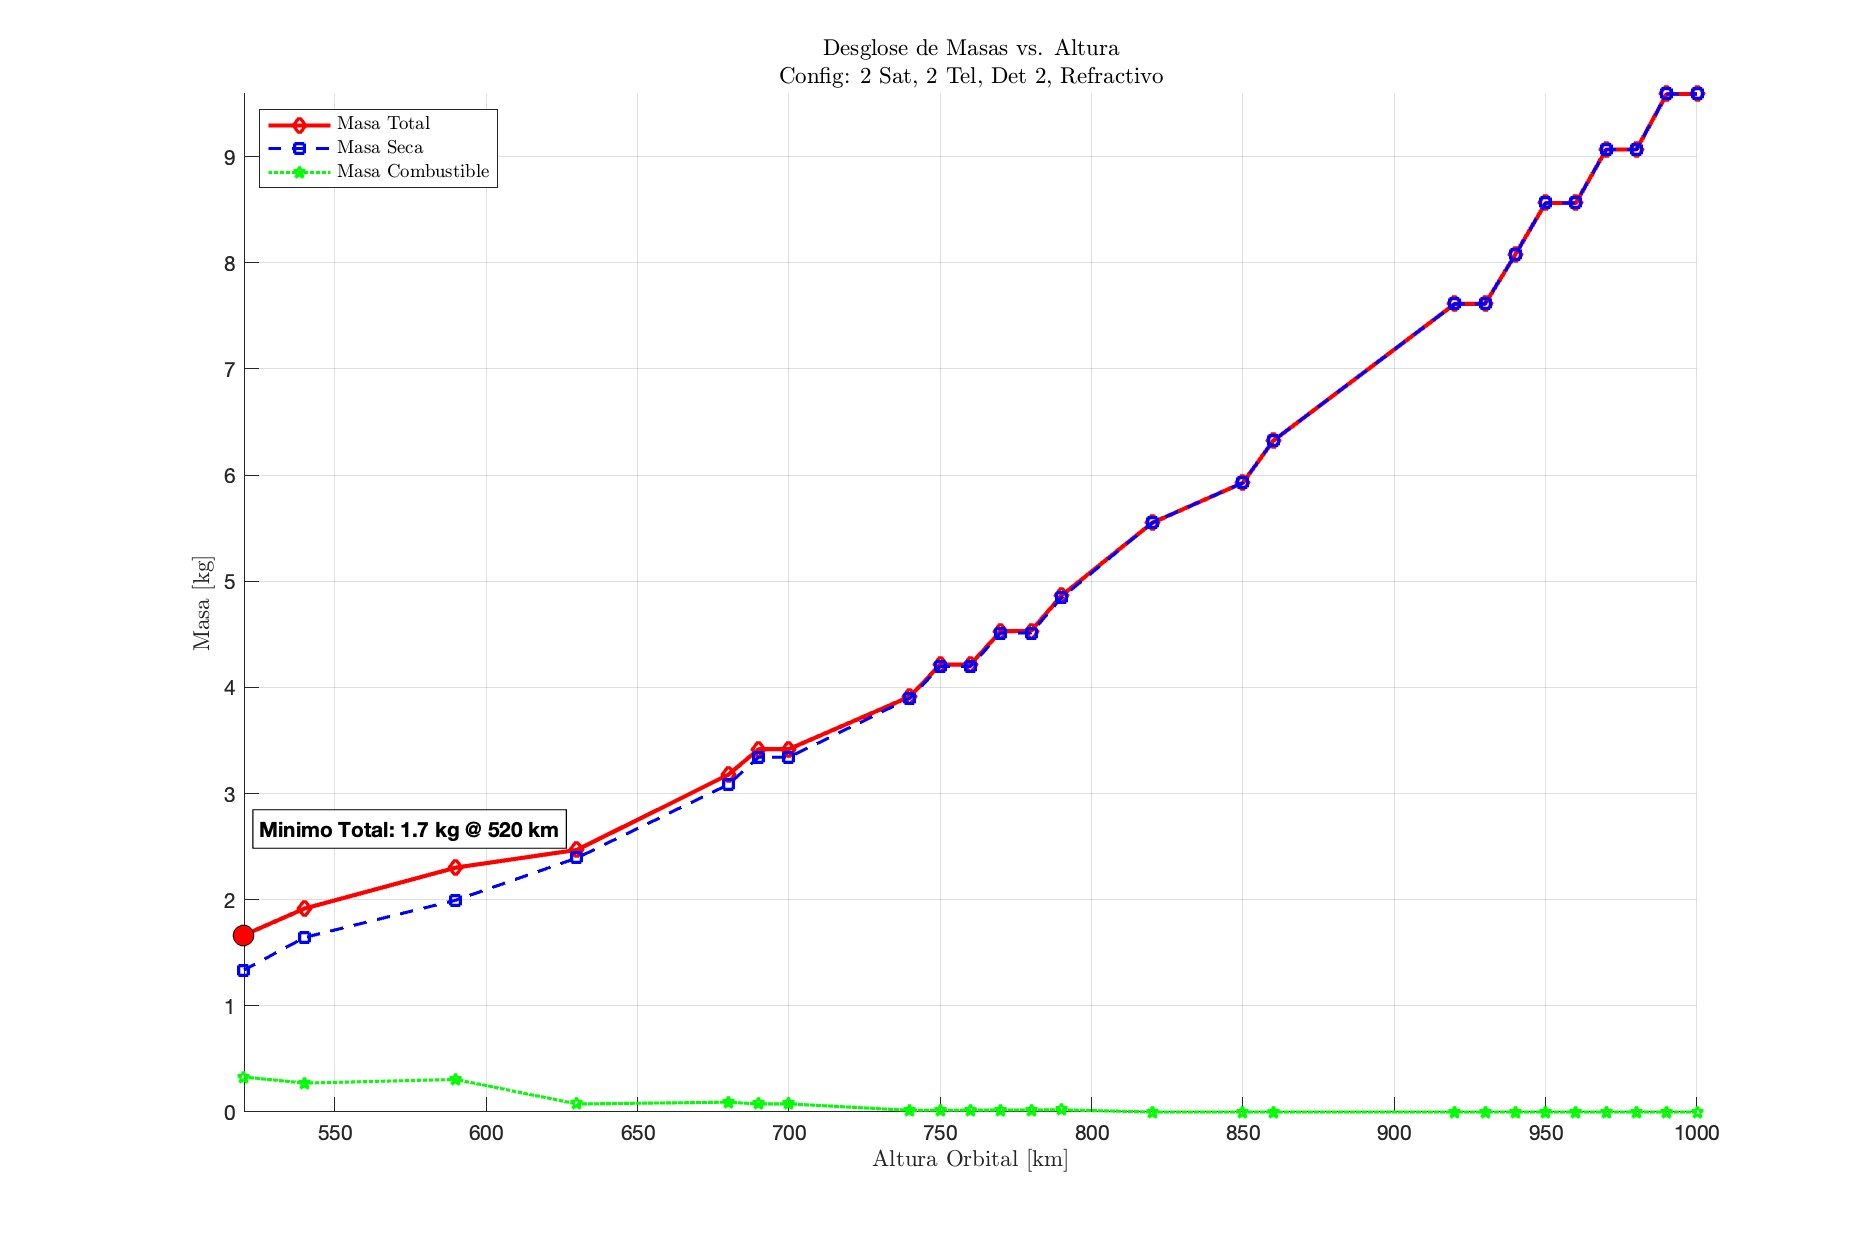
\includegraphics[width=1\linewidth]{5.Mission/MasaDesglose_2sat_2tel_Det2_Refractivo.jpg}
    \caption{Desglose de masa seca, masa combustible y masa total. \\Fuente: Elaboración propia.}
\end{figure}

Apreciando en esta gráfica el mínimo de masa a poner en orbita por satélite de \textbf{1,67 kg} (distribuidos como: $m_{seca}= 1,34\ kg; \quad m_{comb}= 0,33 kg$) a una altura orbital de \textbf{520 km}, correspondiente a un diámetro de pupila de \textbf{28 mm}. Dado que la constelación estará formada por dos satélites, la masa total a inyectar en orbita será de \textbf{3,34 kg}.

Las instrumentación del satélite final, calculando los parámetros restantes descritos previamente, será dispuesto de la siguiente manera:
\begin{landscape}
\begin{figure}[H]
    \centering
    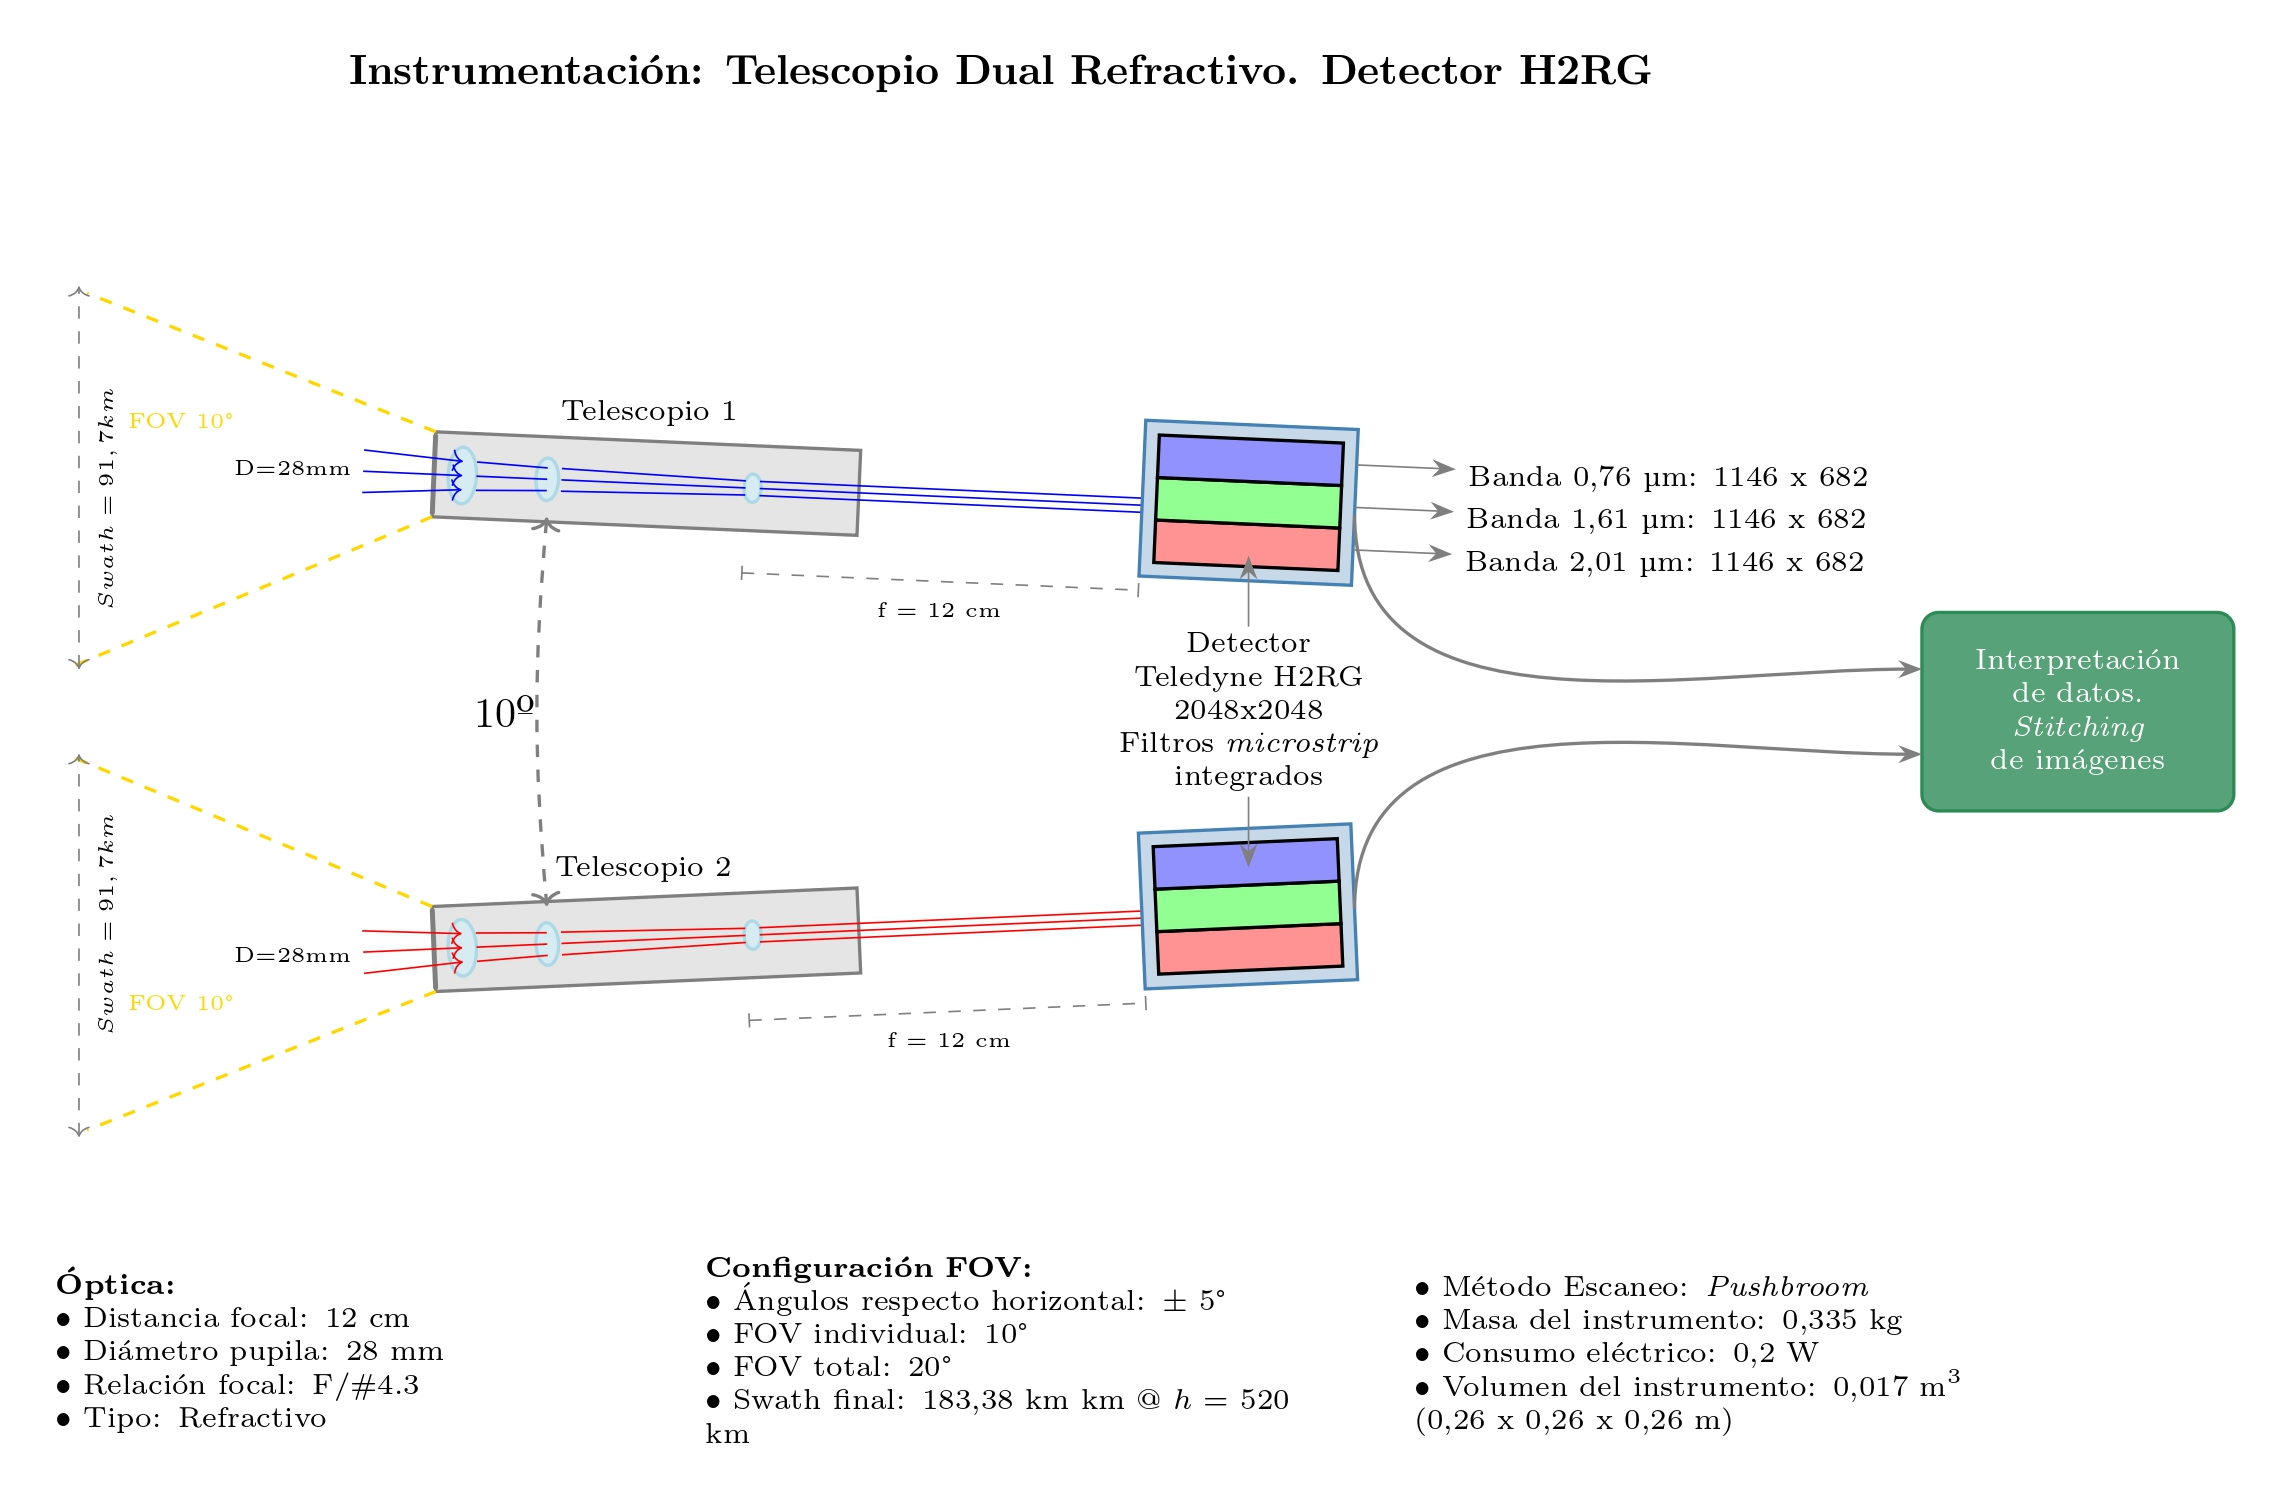
\includegraphics[width=1\linewidth]{5.Mission/TFG_Tikz-8.jpg}
    \caption{Esquemática de la carga de pago final. \\ Fuente: Elaboración propia.}
    \label{fig:enter-label}
\end{figure}
\end{landscape}

\begin{figure}[H]
    \centering
    \begin{subfigure}[b]{0.3\textwidth}
        \centering
        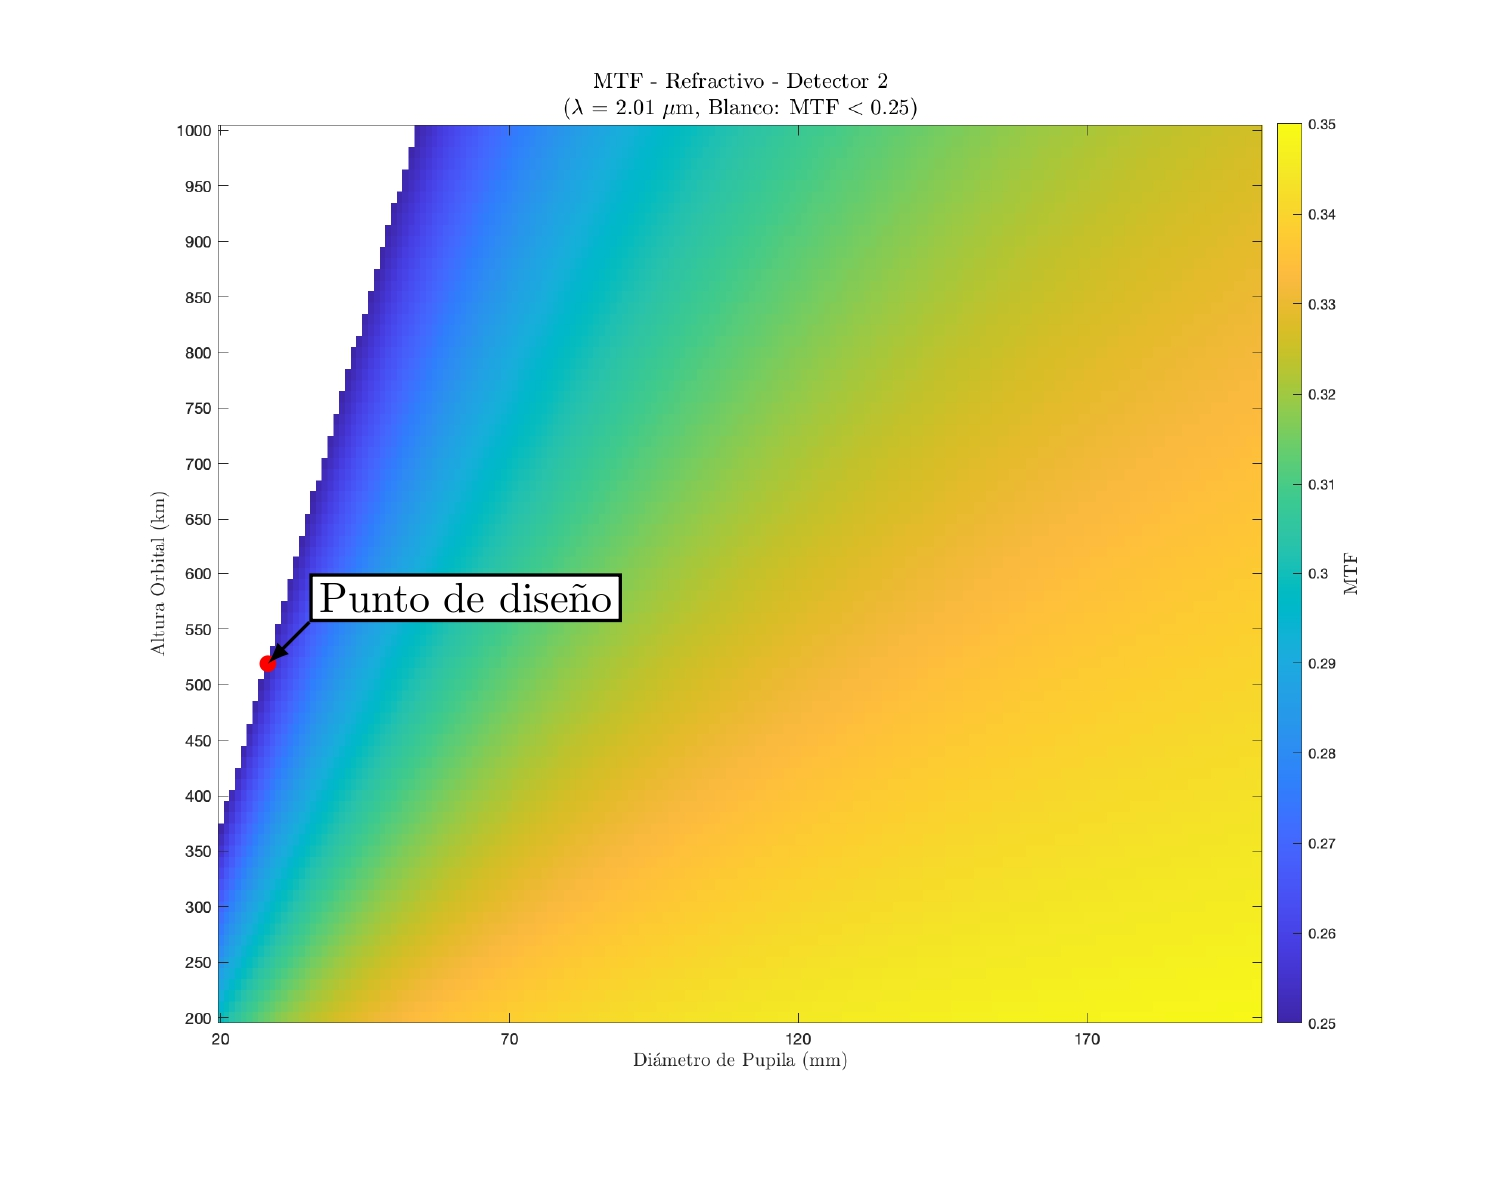
\includegraphics[width=\textwidth]{5.Mission/TFG_Tikz-4.jpg}
        \caption{MTF en banda $2,01\ \mu m$}
        \label{fig:sub1}
    \end{subfigure}
    \hfill
    \begin{subfigure}[b]{0.3\textwidth}
        \centering
        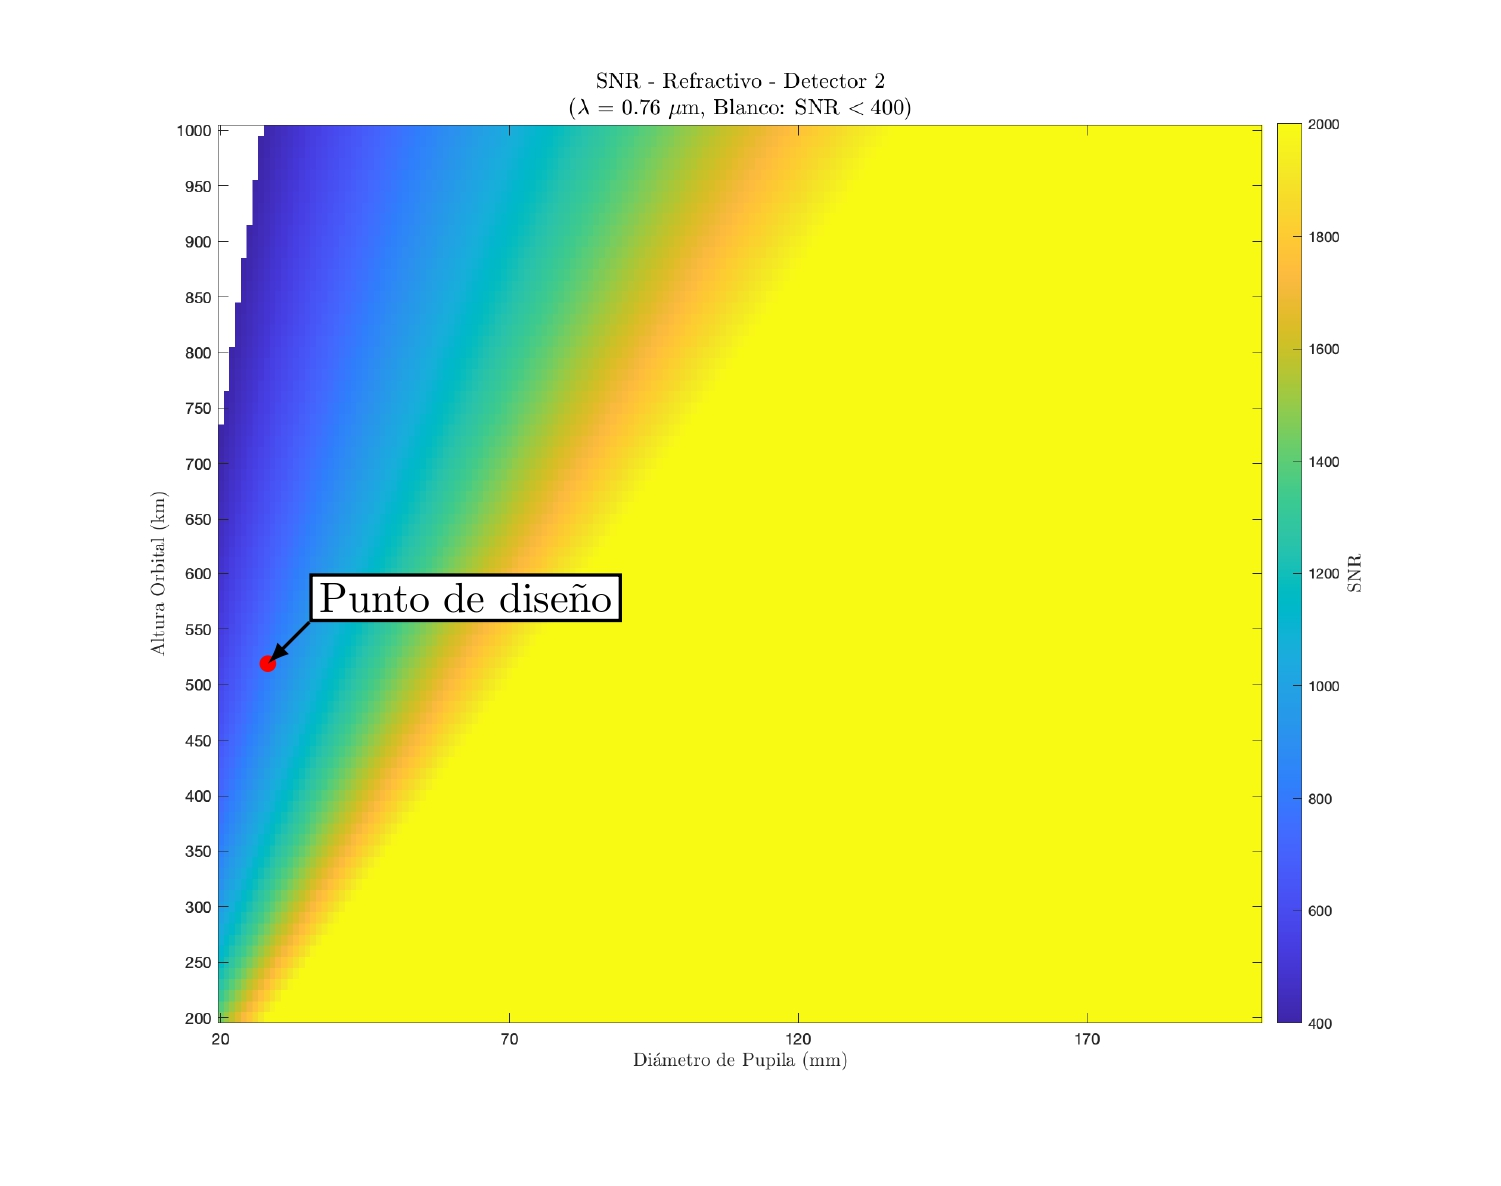
\includegraphics[width=\textwidth]{5.Mission/TFG_Tikz-5.jpg}
        \caption{SNR en banda $0,76\ \mu m$}
        \label{fig:sub2}
    \end{subfigure}
    \hfill
    \begin{subfigure}[b]{0.33\textwidth}
        \centering
        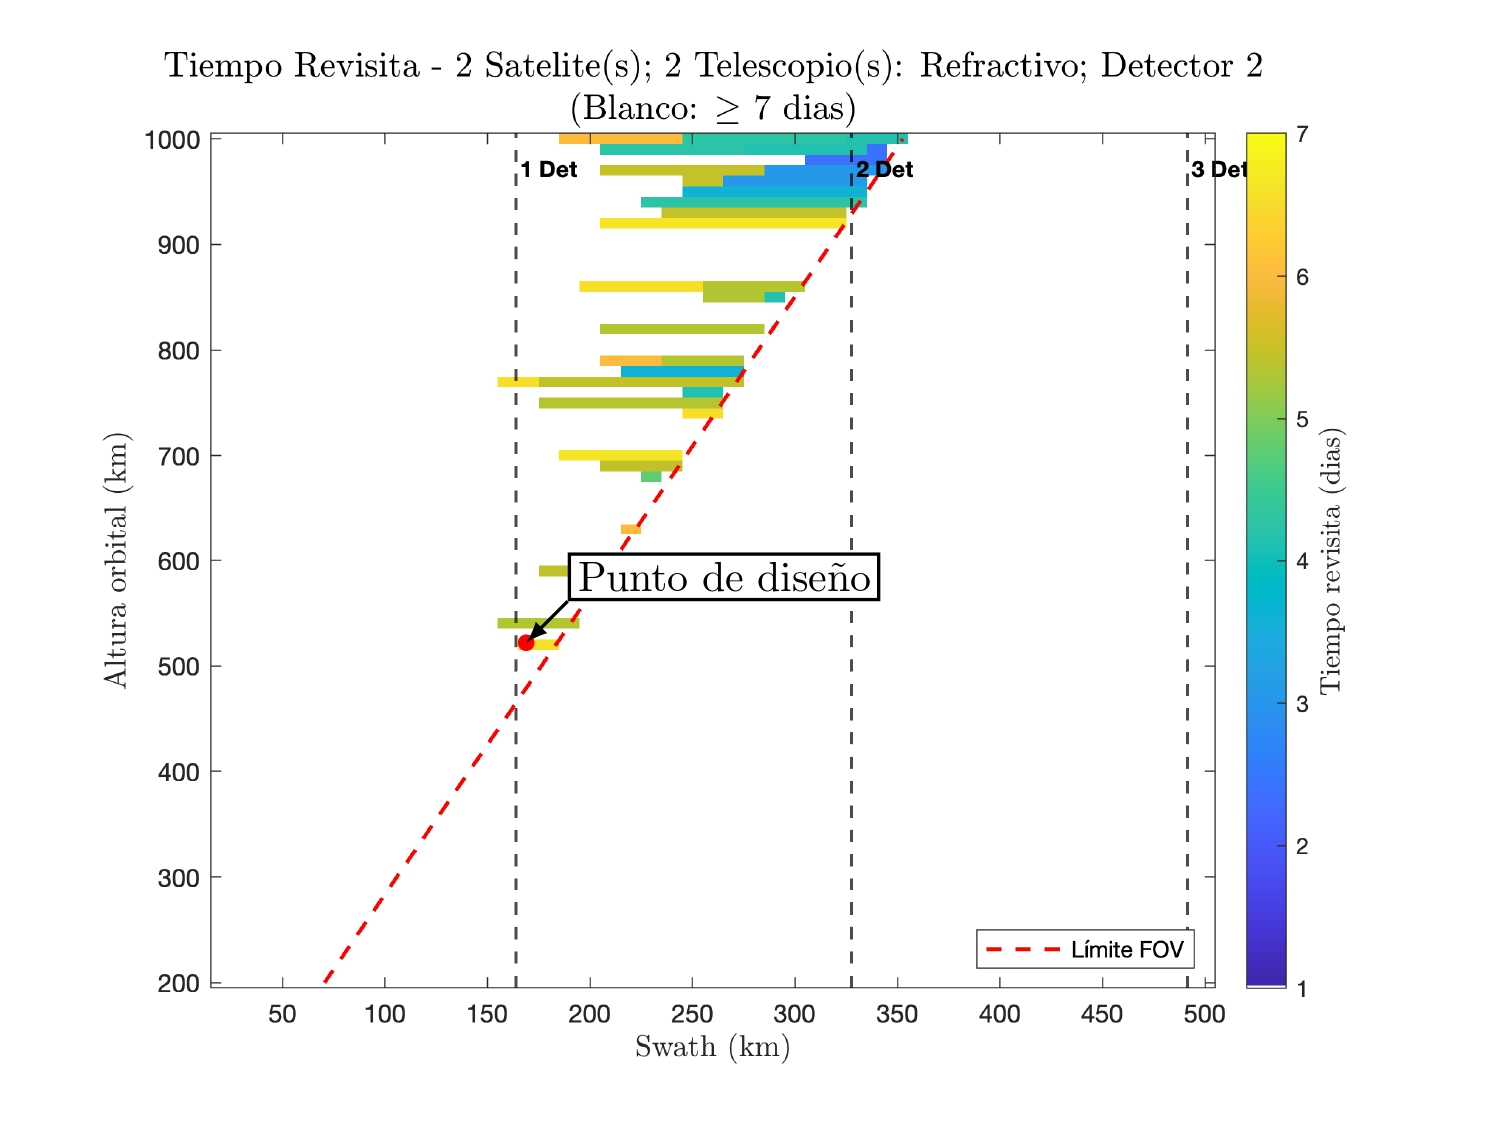
\includegraphics[width=\textwidth]{5.Mission/TFG_Tikz-6.jpg}
        \caption{Cobertura de la región}
        \label{fig:sub3}
    \end{subfigure}
    \caption{Punto de diseño del satélite. \\ Fuente: Elaboración propia.}
    \label{fig:puntodiseno}
\end{figure}

Dado que el swath requerido es de 170 km, mientras el swath final obtenido es de 183 km, se consigue un solapamiento final del 10\%, añadiendo a nuestro requerimiento mínimo. La restricción es impuesta por el fov combinado de los telescopios. Debido a que el \textit{swath} completo de un detector individual es de $2048*80= 163 km$, y el fov de un telescopio único limita a $ 91 km$, solo podrán usarse 1146 pixeles de ancho.

En el anexo \ref{sec:annexdata}, se podrán encontrar las masas totales de las soluciones viables que aporta cada combinación de configuración, telescopio y detector, siendo la presentada en este capitulo el mínimo de masa absoluto a poner en órbita.


\subsection{Fin de misión}

La gestión de los desechos orbitales supone en la actualidad un aspecto a considerar, dada la creciente preocupación por la sostenibilidad del entorno espacial. Con el objetivo de mitigar el impacto negativo de la basura espacial, resulta interesante evaluar la necesidad de implementar maniobras activas para garantizar la reentrada controlada de los satélites una vez finalizada su misión. En este contexto, se considera razonable que el tiempo transcurrido desde el fin de operaciones hasta la reentrada en la atmósfera terrestre sea inferior a \textbf{un año}, especialmente para artefactos situados en órbitas LEO \cite{nasa_deorbit_systems_2025}.


\begin{figure}[H]
    \centering
    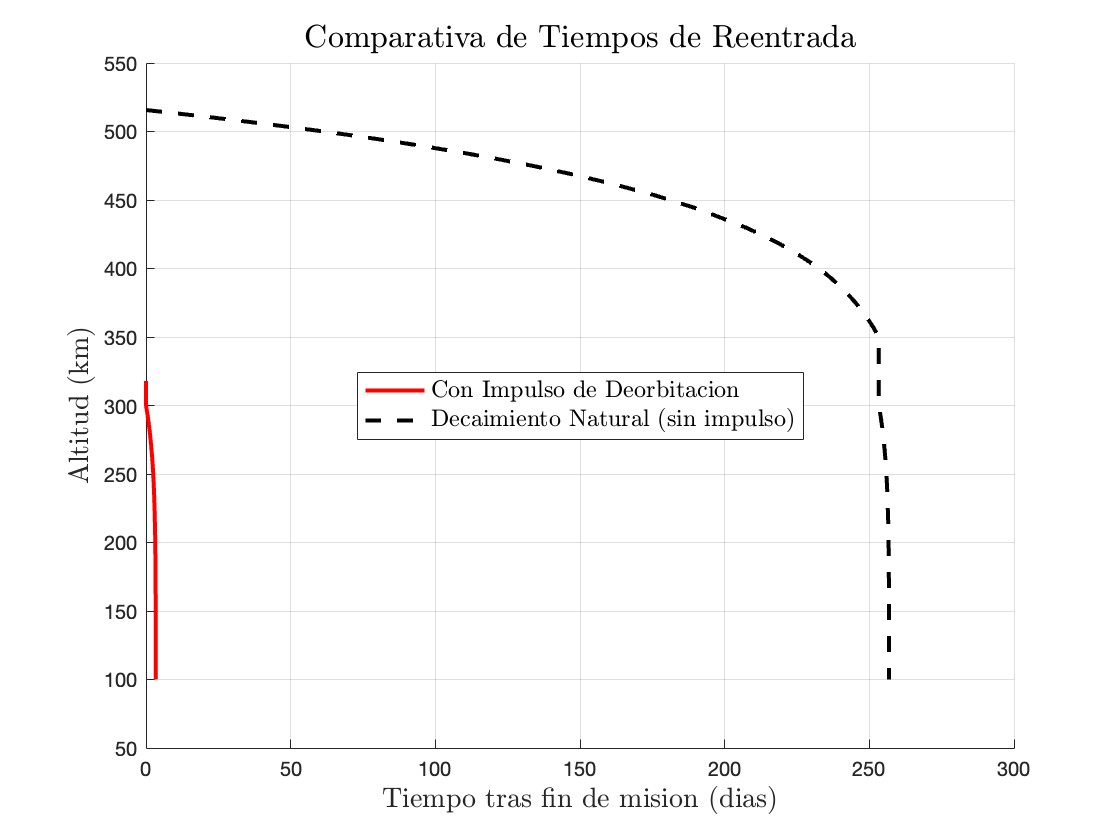
\includegraphics[width=1\linewidth]{5.Mission/deorbit.jpg}
    \caption{Tiempo de deorbitación, en días, tras fin de misión. \\Fuente: Elaboración propia.}
\end{figure}

En el caso analizado, la simulación del tiempo de reentrada a la altitud seleccionada indica que los satélites tardarían aproximadamente \textbf{257 días} en descender de manera natural. Este valor se encuentra dentro del intervalo considerado como aceptable. Por tanto, no será necesario incrementar la masa de combustible destinada a maniobras de deorbitación.


\chapter{Subsistemas}

En este capítulo, una vez definido el instrumento, se va a desarrollar brevemente el conjunto del satélite. En base a los datos de masa y volumen totales se podrá definir los subsistemas que acompañan a la carga de pago y hacen posible la misión. Se elegirán componentes comercialmente disponibles (\textit{off-the-shelf}) para así validar nuestra solución. Ya que el satélite entra en la categoría de nanosatélites (entre 1 y 10 kg), se tomarán referencias y documentaciones previas sobre este tipo de vehículos. A continuación se presenta el desglose de masas. En las secciones subsiguientes, se procederá al análisis pormenorizado de cada uno de los subsistemas que componen el vehículo: 

%% TABLA
\begin{table}[h]
  \centering
  \caption{Distribución de masa por subsistema}
  \begin{tabular}{@{}l S[table-format=1.3] S[table-format=2.1]@{}}
    \toprule
    Subsistema                               & {Masa (kg)} & {Porcentaje (\%)} \\
    \midrule
    Instrumento de observación               & 0,335    & 20,1        \\
    Subsistema eléctrico                     & 0,269    & 16,1           \\
    \midrule
    \quad Paneles solares                    & 0,229    & 13,7         \\
    \quad Baterías                           & 0,040    & 2,4          \\
    \midrule
    Comunicaciones (banda X)                 & 0,270    & 16,2          \\
    Estructura                               & 0,251    & 15,0          \\
    Control de actitud                       & 0,050    & 3,0           \\
    Propulsión                               & 0,057    & 3,4          \\
    \midrule
    \quad Motor                          & 0,040    & 2,4         \\
    \quad Depósito                           & 0,017    & 1,0           \\
    \midrule
    Ordenador de a bordo (OBC)               & 0,094    & 5,6          \\
    Gestión térmica                          & 0,050    & 3,0          \\
    \midrule
    \textbf{Total masa seca}                 & \textbf{1,336} & \textbf{80,0}  \\
    \textbf{Combustible}                     & \textbf{0,334} & \textbf{20,0}  \\
    \textbf{Masa total}                      & \textbf{1,670}  & \textbf{100,0} \\
    \bottomrule
  \end{tabular}
\end{table}




\section{Estructura}

La estructura forma el elemento estructural del satélite, donde se acoplarán el resto de módulos. Su diseño debe permitir soportar las cargas mecánicas durante el lanzamiento, tanto en fuerzas de aceleración longitudinales, laterales, como en vibraciones, a medida que el lanzador asciende. Una de las opciones más comunes para su fabricación en este tipo de satélites supone usar un chasis de aleaciones de aluminio como 6061-T6 y 7075-T6.

La masa estructural representa típicamente entre 15-20 \% de la masa total del satélite \cite{tsinas2001efficient}. Este porcentaje se mantiene relativamente constante debido a la escalabilidad de las cargas estructurales. Por tanto, se puede asumir que la masa estructural del satélite será de 0,251 kg (15\%).


\section{Control de Actitud}

El subsistema de control de actitud (ADCS) tiene como misión mantener la orientación del satélite en todo momento, para que el instrumento siempre apunte al nadir y los paneles solares queden siempre correctamente orientados. También debe compensar perturbaciones externas como el gradiente gravitatorio, la presión de radiación solar, el arrastre atmosférico y las variaciones del campo magnético terrestre; además de realizar el apuntamiento del motor en las maniobras de propulsión.

\begin{figure}[H]
    \centering
    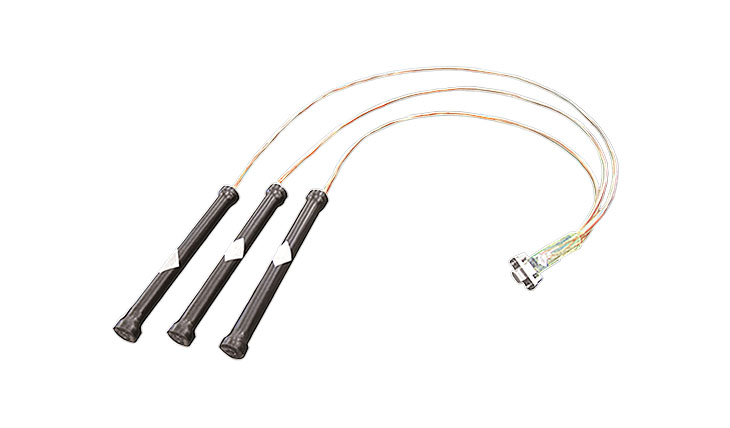
\includegraphics[width=0.5\linewidth]{5.Mission/featured_image.jpg}
    \caption{Magnetotorque GMAT-1. \\Fuente: \cite{satcatalog:gmat1}}
\end{figure}

Para satisfacer estos requisitos, se selecciona un sistema de control basado exclusivamente en magnetopares triaxiales, integrados en un único módulo: \textbf{GMAT-1}, del fabricante\textbf{ Michigan Aerospace Manufacturers Association}. Este sistema incluye un magnetómetro para la medición precisa del campo magnético terrestre y algoritmos de control embebidos. La elección de magnetopares responde a criterios de simplicidad, bajo consumo, mínimo volumen y masa, y capacidad suficiente para mantener el apuntamiento nadir. Su consumo máximo es de 0,25 W, y con una masa de 0,05 kg, representa aproximadamente el 6\% de la masa total del satélite \cite{satcatalog:gmat1}.

\section{Comunicaciones}

El subsistema de comunicaciones se basa exclusivamente en usar una de la bandas más comunes para este tipo de aplicaciones, la banda X. Este protocolo tiene capacidad suficiente para la descarga de las imágenes captadas por el instrumento de observación, así como recibir y envíar datos de telemetría y telecomando. La selección de componentes se basa en módulos comerciales de alta fiabilidad. Mientras otras configuraciones ofrecen soluciones multibanda (Ka, Ku, S y X), la restricción de peso obliga a utilizar un solo transmisor lo más liviano posible. Como se detalla en el capítulo \ref{tierra}, esta banda será más que suficiente para cumplir la misión.

\begin{figure}[H]
    \centering
    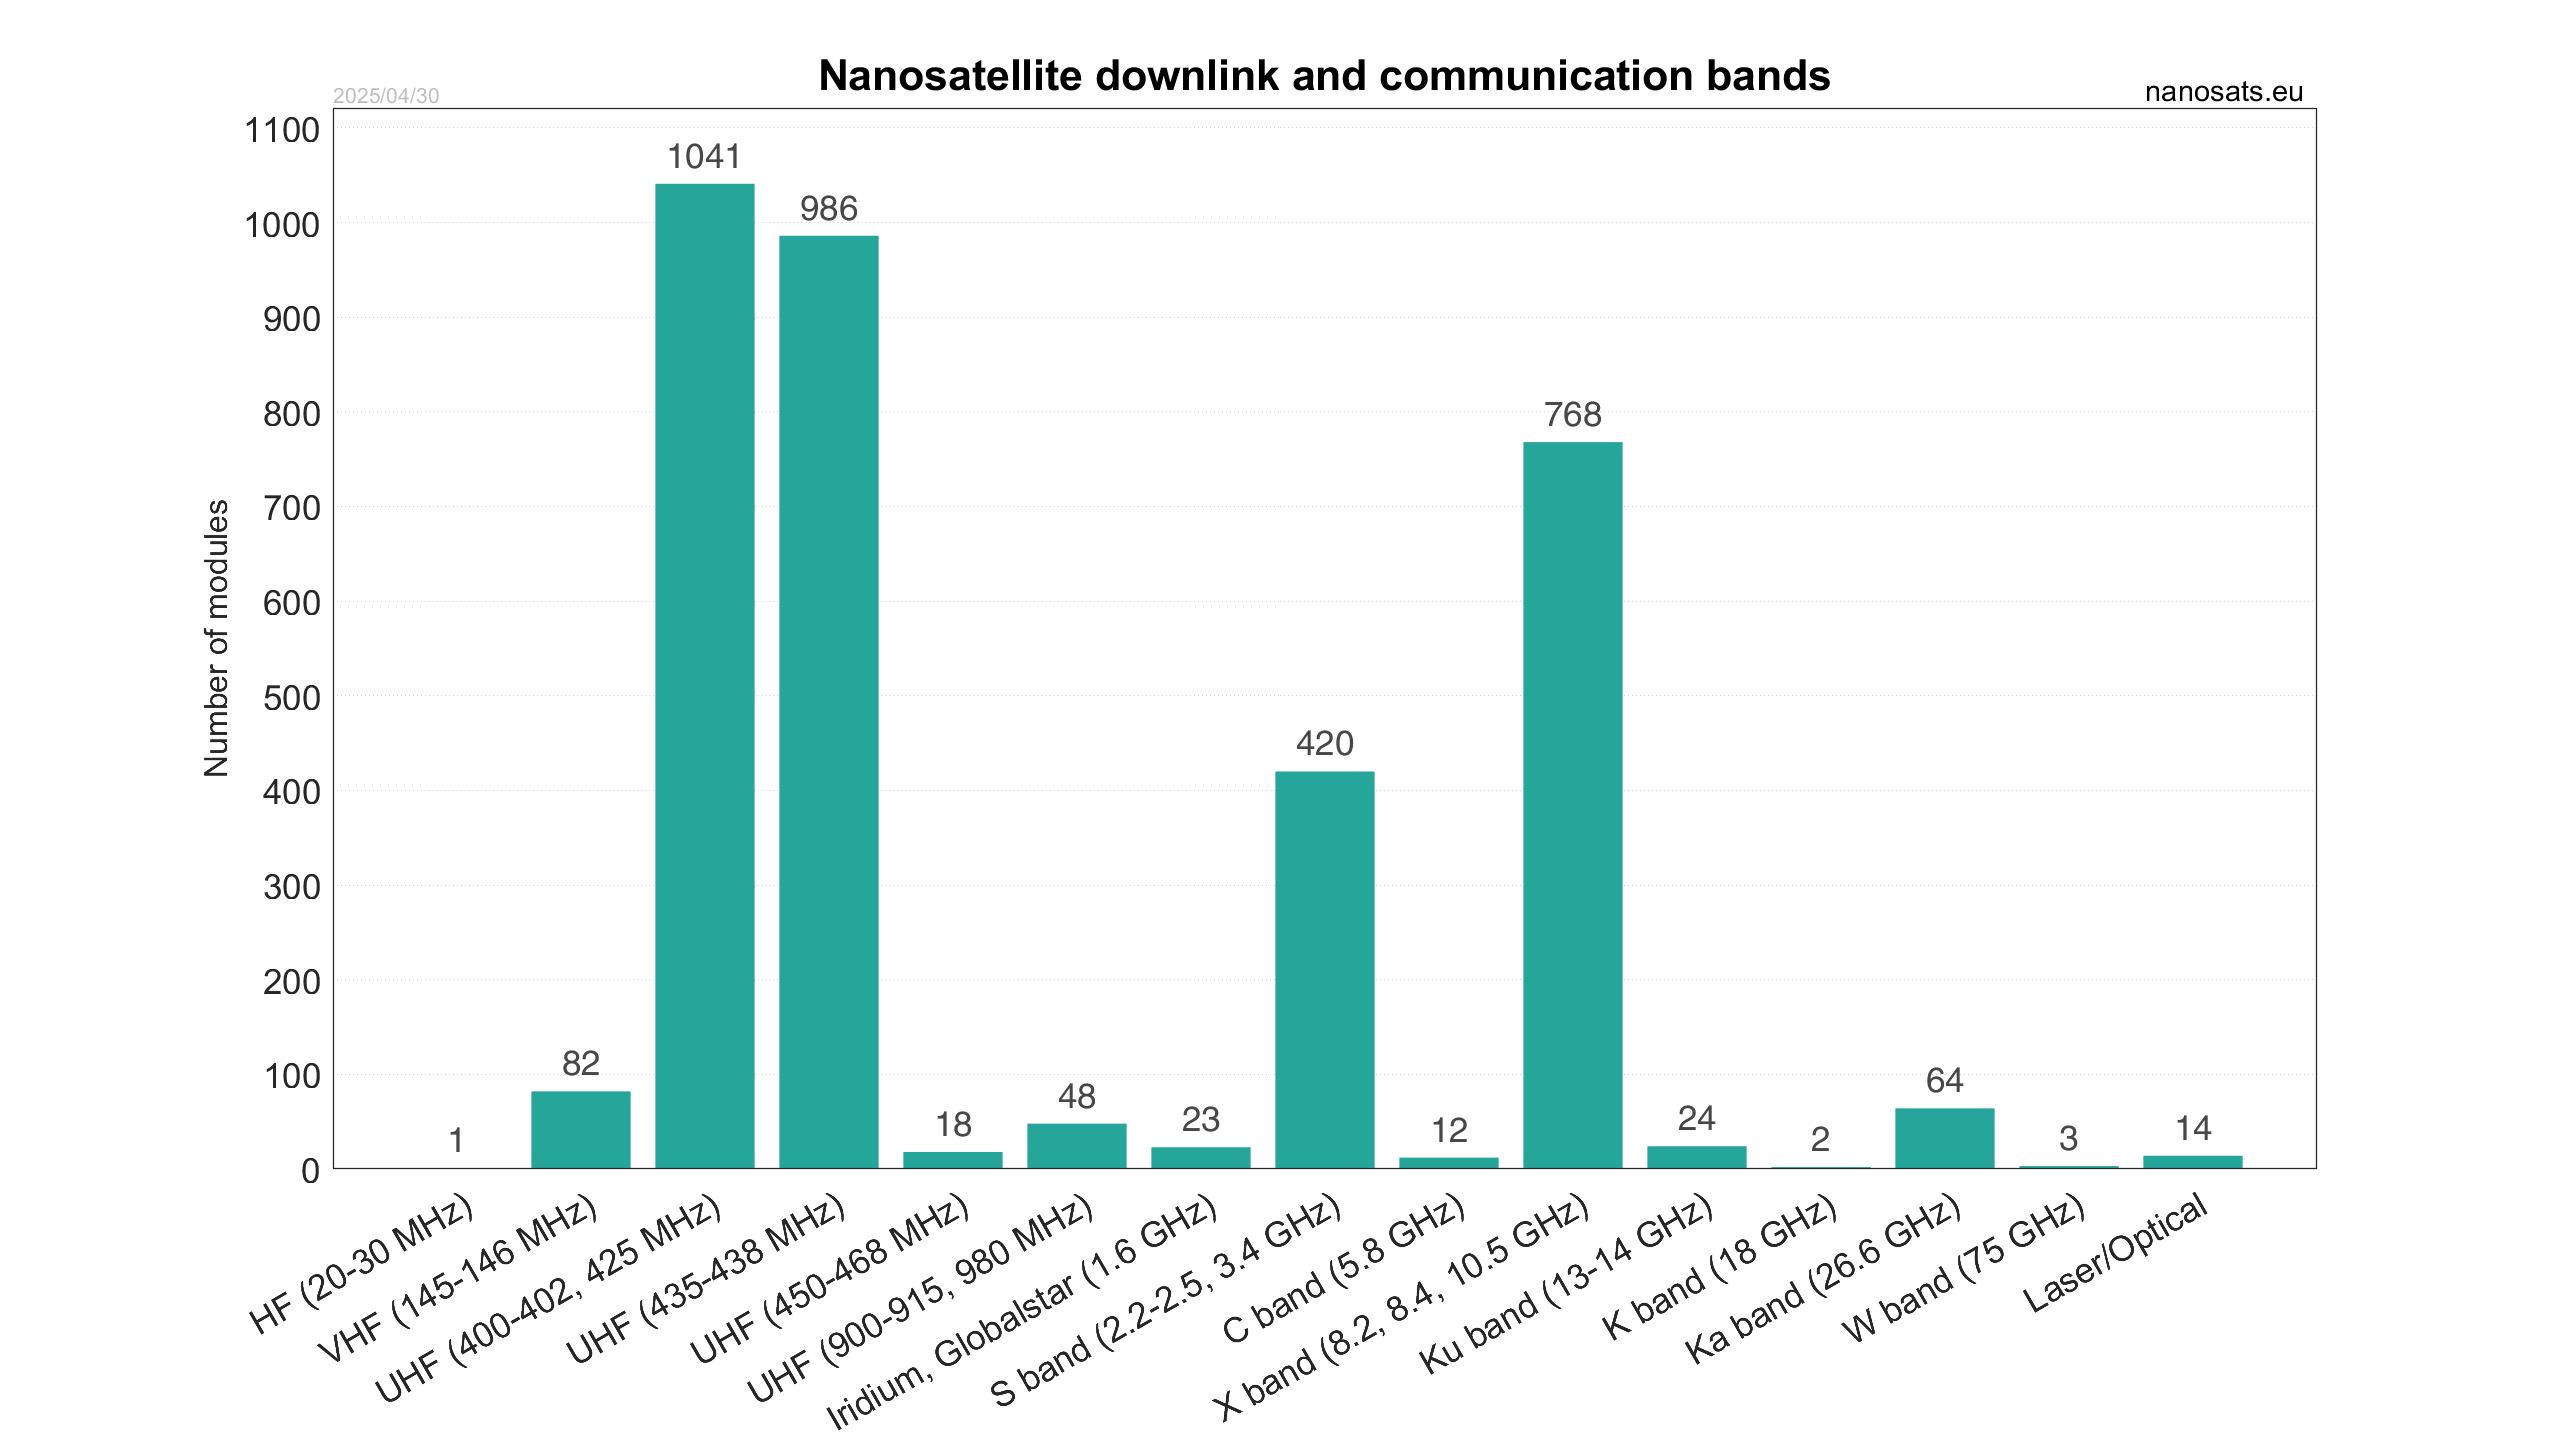
\includegraphics[width=0.7\linewidth]{5.Mission/Nanosats_frequency_2025-04-30_large.png}
    \caption{Bandas de de comunicaciones de uso típico en nanosatélites.  \\Fuente: \cite{kulu2025nanosats}}
\end{figure}


 Para las comunicaciones, se ha seleccionado un transmisor en banda X modelo \textbf{X-Band del fabricante EnduroSat}. Este dispositivo opera en el rango de frecuencias comprendido entre 8,000y 8,400 GHz, permitiendo una tasa de transmisión de datos media de 150 Mbps. La potencia de salida es de 2 W, con un consumo eléctrico en transmisión de 22 W y una masa aproximada de 270 g \cite{endurosat_xband_2025}.

Por tanto, el sistema de comunicaciones suma 270 g, o un \% de la masa total.

\section{Subsistema eléctrico}

El subsistema eléctrico, se encarga de generar, almacenar, acondicionar y distribuir la energía eléctrica que requieren todos los componentes del satélite para su operación. Para dimensionarlo, se puede realizar un presupuesto de potencia. En él, se considerarán 3 modos de operación:

\begin{itemize}
    \item Toma de datos activa: Corresponde a la operación nominal del instrumento. Los consumos son: instrumento (\SI{0,2}{W}), sistema de control de actitud o ACDS (\SI{0,25}{W}) y el ordenador de a bordo u OBC\footnote{El \textit{On Board Computer} (Ordenador de Abordo), se define más adelante.} (\SI{0,4}{W}). El consumo total en este modo es de \textbf{\SI{0,85}{W}}
    \item \textit{Standby} o hibernación: Modo de bajo consumo para los periodos de inactividad. Los sistemas activos son: ACDS en modo mantenimiento (\SI{0,05}{W}) y OBC (\SI{0,4}{W}). El consumo total en este modo es de \textbf{\SI{0,45}{W}}.
    \item Transmisión de datos: Es el modo de mayor demanda energética, activado para la descarga de datos a la estación de Tierra. Los consumos son: transmisor EnduroSat X-Band (\SI{20}{W}), instrumento (\SI{0,2}{W}), ACDS (\SI{0,25}{W}) y OBC (\SI{0,4}{W}). El consumo total en este modo asciende a \textbf{\SI{20,85}{W}}.
\end{itemize}

\subsubsection{Dimensionado de los paneles}

La generación de potencia se basa en la conversión de la energía solar mediante células fotovoltaicas. La principal métrica para el dimensionado es la irradiancia solar, que es la potencia por unidad de superficie que incide sobre la atmósfera terrestre, con un valor estándar aproximado de \(\SI{1361}{W/m^2}\). Asumiendo una eficiencia de conversión del 20\% ,se aplica un factor de pérdidas y degradación del 0,8 para tener en cuenta efectos como la temperatura y el ángulo de incidencia\cite{nasa2025power}. Con estos parámetros, la potencia específica que se puede generar es:
\[
P_{\text{específica}} = \SI{1361}{W/m^2} \times 0,20 \times 0,8 = \SI{217,8}{W/m^2}
\]
Para minimizar la masa, se opta por una tecnología de paneles solares flexibles, que presentan una menor densidad másica. Conforme al presupuesto de masas, se asigna un total de \textbf{\SI{0,229}{kg}} para los paneles. Considerando una densidad de \(\SI{4}{kg/m^2}\) para este tipo de tecnología, el área disponible es de \SI{0,057}{m^2}\cite{hiansa2022panel}. A partir de esta superficie, la potencia total generada por el subsistema es:
\[
P_{\text{generada}} = P_{\text{específica}} \times A_{\text{panel}} = \SI{217,8}{W/m^2} \times \SI{0,057}{m^2} \approx \textbf{\SI{12,47}{W}}
\]
Esta potencia es suficiente para alimentar los modos de operación nominales y permitir la recarga de las baterías.

\subsubsection{Dimensionado de baterías}

Las baterías de iones de litio se dimensionan para suplir el déficit energético durante el modo de transmisión, que presenta el mayor consumo. El déficit de potencia a cubrir es de \(\SI{20,85}{W} - \SI{12,47}{W} = \SI{8,38}{W}\).

Considerando una duración de transmisión acumulada de 1 hora por día aproximadamente, la energía requerida de la batería es de aproximadamente \SI{8,38}{Wh}. Con una densidad energética de \(\SI{200}{Wh/kg}\), la masa necesaria para el almacenamiento es de \textbf{\SI{0,029}{kg}}\cite{sunket2025lithium}.

La masa total del subsistema eléctrico resultante (\(m_{\text{panel}} + m_{\text{batería}}\)) asciende a \SI{0,258}{kg}. Este valor es consistente con la asignación inicial del presupuesto de masas, validando la configuración propuesta. Considerando que los requerimientos de potencia son laxos, pues el tiempo de transmisión de datos en continuo nunca superará más de los 15 minutos, y el satélite nunca entrará en un eclipse, el dimensionado supone una aproximación favorable a lo esperado en la práctica.


\section{Dimensionado de la planta de potencia}

El subsistema de propulsión constituye un elemento critico para el mantenimiento orbital. La selección del sistema propulsivo debe considerar tanto los requerimientos de impulso especifico como las limitaciones de masa y volumen propias de los nanosatélites. Una de las opciones m\'as innovadoras que comprenden este tipo de vehículos es el uso de motores monopropelentes de combustible verde no toxico. Esto simplifica el diseño al no necesitar 2 depósitos, reduce los riesgos de manipulación y consigue re-encendidos tras a\~nos en \'orbita, manteniendo un impulso especifico competitivo. Por tanto, se escoge el propulsor \textbf{100mN HPGP THRUSTER} desarrollado por ECAPS. Este sistema presenta las características técnicas que satisfacen los requerimientos operacionales:

\begin{itemize}
    \item Empuje nominal: 100 mN con rango operacional de 30-100 mN
    \item Impulso especifico: 209 s nominal
    \item Masa del propulsor: 40 g
\end{itemize}

El sistema incorpora combustible LMP-103S, que proporciona hasta 30\% mejor rendimiento por volumen comparado con hidracina tradicional. El propulsor incluye sistema de precalentamiento del reactor y elementos térmicos esenciales para arranques en frío durante la misión, garantizando el encendido tras los 8 años de operación \cite{ECAPS_100mN_HPGP}.

\subsubsection{Depósito de combustible}

El dimensionado del sistema de almacenamiento de combustible se basa en análisis de relaciones masa-combustible establecidas para sistemas espaciales. Para tanques de hidrazina, la relación masa del tanque respecto al combustible es aproximadamente 0,05 kg por kilogramo de combustible \cite{smad2002spacecraft}.
Con una masa de combustible de 0,334 kg, el tanque requerido presenta:
\begin{equation}
M_{\text{tanque}} = 0,334 \times 0,05 = 0,0167\text{kg}
\end{equation}

Por tanto la masa total del subsistema será de: 
\begin{align}
    0,014 + 0,040 = 0,0567\ kg
\end{align}
Esto supone aproximadamente un 4 \% de la masa total del satélite.

\subsection{Otros subsistemas adicionales}
\subsubsection{Ordenador de Abordo (\textit{On Board Computer}, OBC)}

El ordenador de a bordo (OBC) se encarga de la gestión centralizada de datos, el control de los subsistemas y la ejecución de los algoritmos de misión, garantizando la fiabilidad mediante redundancias y arquitectura tolerante a fallos. El seleccionado para el satélite es el modelo \textbf{iOBC de ISISPACE}. Este equipo presenta una masa de 0,094 kg y un consumo medio de potencia de 0,4 W. Su peso supone aproximadamente un 3\% de la masa total del satélite \cite{isisobc}.


\subsubsection{Gestión térmica}

El subsistema de gestión térmica se basa en una arquitectura pasiva, empleando recubrimientos de control térmico, disipadores y aislamiento. Esta solución minimiza el consumo energético y el numero de componentes. La masa total estimada es de un 3\% o  0,05 kg, incluyendo recubrimientos, adhesivos, aislamiento y elementos de interfaz térmica \cite{guzman2025thermal} \cite{nasa2025thermal}.